\documentclass{llncs}
\usepackage[utf8]{inputenc}
\usepackage[spanish]{babel}
\usepackage{graphicx}
\usepackage{listings}
\usepackage{xcolor}
\usepackage{amsmath}
\usepackage{hyperref}

\hypersetup{
    colorlinks=true,
    urlcolor=blue
}

\lstset{
    basicstyle=\ttfamily\footnotesize,
    breaklines=true,
    frame=single,
    numbers=left,
    keywordstyle=\color{blue},
    commentstyle=\color{gray},
}

% Configuración de encabezados y pies de página
\pagestyle{headings}
\title{Proyecto Final de Compilación: Diseño e Implementación de un Compilador para el Lenguaje HULK}
\author{Claudia Hernández Pérez \and Joel Aparicio Tamayo \and Kendry J. Del Pino Barbosa}
\institute{Facultad de Matemática y Computación, Universidad de La Habana} 

\begin{document}

\maketitle

\begin{abstract}
Este documento describe el diseño e implementación de un compilador para HULK en el lenguaje C. El 
diseño del compilador agrupa 4 partes: \textit{lexer}, \textit{parser}, \textit{chequeo semántico} y \textit{generación de código}.

El \textit{lexer} y el \textit{parser} se basan en los frameworks proporcionados por \texttt{Lex} y \texttt{Yacc}, respectivamente, aunque el proyecto cuenta con
una implementación propia de un \textit{lexer} basado en la teoría de autómatas finitos. El \textit{chequeo semántico} es responsable de validar las reglas del lenguaje,
reduciendo los errores en tiempo de ejecución. Para ello se ha implementado el patrón Visitor, que permite recorrer el árbol de sintaxis abstracta (AST) y aplicar las reglas semánticas correspondientes. Además,
cuenta con una arquitectura que permite la unificación de expresiones con tipos, lo que facilita la inferencia. Finalmente, la \textit{generación de código} se realiza mediante un generador de código intermedio que
también implementa el patrón Visitor para traducir el AST a código LLVM.

Al ejecutar el compilador de HULK, se genera un \texttt{output.ll} en la carpeta \textit{build}, donde se encuentra 
el código generado, y luego se invoca al compilador de LLVM para ejecutar dicho archivo, y devolver la salida del programa.
\vspace{10pt}
\keywords{Compilador \and Lexer \and Parser \and Chequeo Semántico \and AST \and Scope \and Generación de código \and LLVM \and Inferencia \and Expresión \and Tipo}
\end{abstract}

\section{Introducción}
Los compiladores son herramientas fundamentales en la ciencia computacional, actuando como puentes entre abstracciones de alto nivel y ejecución eficiente. Específicamente, HULK (Havana University Language for Kompilers),
es un lenguaje de programación didáctico, seguro de tipos, orientado a objetos e incremental. Este proyecto tiene la finalidad de compilar un subconjunto de dicho 
lenguaje, siendo consistente con las especificaciones en su \href{https://matcom.in/hulk/guide/intro}{definición formal}, aunque añadiendo algunas extensiones sintácticas propias.

Para compilar HULK, se ha diseñado un flujo de trabajo sencillo y por capas. El punto de entrada del programa es 
el archivo \texttt{main.c}, que intenta leer un archivo \texttt{script.hulk} en formato de cadena de texto y luego invoca al \textit{lexer} y al \textit{parser} para generar un árbol de sintaxis abstracta (AST). Posteriormente,
si no hubo errores léxicos ni sintácticos, se realiza el \textit{chequeo semántico} a partir del nodo raíz del AST. Finalmente, si no hubo errores semánticos, se procede a la \textit{generación de código} intermedio, que se traduce a código LLVM. En
este punto concluye el proceso de compilación, generando un archivo \texttt{output.ll} en la carpeta \textit{build}. Para cada proceso del programa (compilación, ejecución, limpieza) existe una receta en el \texttt{Makefile} que lo ejecuta: 
\begin{lstlisting}[language=bash]
make compile // para compilar y generar el build/outout.ll
make execute // para ejecutar el compilador de LLVM 
make clean // para limpiar el directorio de compilacion
\end{lstlisting}

A continuacón se detallan los disitntos aspectos de la implementación.
\vspace{10pt}
\section{Lexer y parser}

Para el \textit{lexer} y el \textit{parser} se ha utilizado el framework proporcionado por \texttt{Lex} y \texttt{Yacc}, aunque se tiene una implementación manual del \textit{lexer} utilizando la teoría de autómatas finitos.

\subsection{Lex. Definición de los tokens}

El \textit{lexer} es el encargado de transformar la entrada del programa (un archivo de texto) en una secuencia de tokens, que son las unidades léxicas del lenguaje. En el programa, los tokens se definen en el archivo \texttt{lexer.l}, 
donde se especifican las expresiones regulares para cada tipo de token.

\textbf{Errores}: En el \textit{lexer} se detecta únicamente un error a la vez, asociados a caracteres inválidos (ver ejemplo Figura~\ref{fig:errores_lex}).
\begin{figure}[h]
\centering
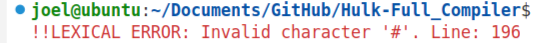
\includegraphics[width=0.7\textwidth]{images/lexer_errors.png}
\caption{Error en lexer}
\label{fig:errores_lex}
\end{figure}

\subsection{Yacc. Definición de la gramática y el AST}
El \textit{parser} es el encargado de analizar la secuencia de tokens generada por el \textit{lexer} y construir un árbol de sintaxis abstracta (AST) a partir de ellos. En el programa, la gramática del lenguaje se define en el archivo \texttt{parser.y}. 
En dicha gramática se definen producciones para cada tipo de \textit{statement} o expresión de HULK, así como una precedencia para los operadores. Cada producción genera un nodo del AST, con lo cual se obtiene finalmente una lista de nodos, que se conectan 
con un nodo raíz, que se hace llamar \textit{program node}.

Existen diversos tipos de nodos que se pueden crear en el parser, cada uno representando una construcción del lenguaje (Ver Figura~\ref{fig:nodos_ast}). Como C no es orientado a objetos, el tipo \texttt{Node} se representa con una estructura que posee campos generales 
que necesitan la gran mayoría de los tipos de nodos, y entre ellos un campo \texttt{data} que es un \textit{union} que tiene las propiedades específicas de cada tipo (Ver Figura~\ref{fig:ast}). Además, existe una función para cada tipo de nodo que permite inicializarlo.

\begin{figure}[h]
\centering
\begin{minipage}{0.3\textwidth}
    \centering
    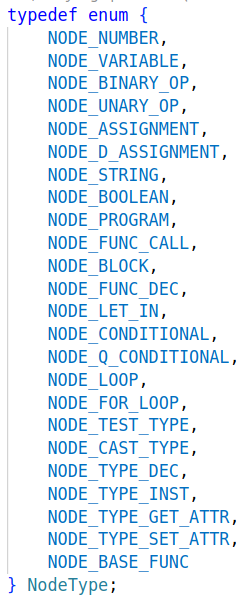
\includegraphics[width=\textwidth]{images/node_type.png}
    \caption{Tipos de nodos del AST}
    \label{fig:nodos_ast}
\end{minipage}\hfill
\begin{minipage}{0.48\textwidth}
    \centering
    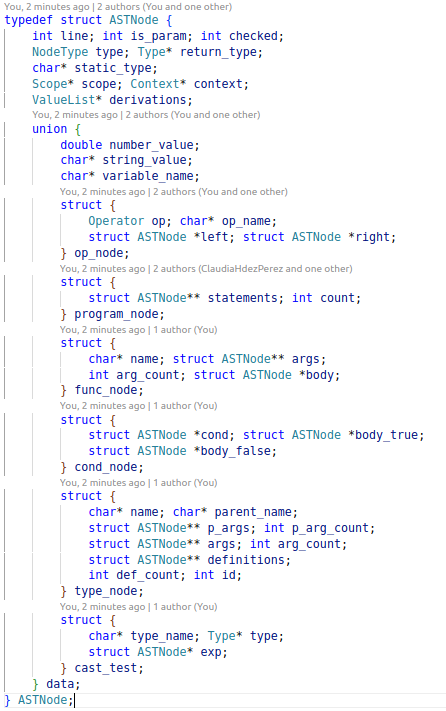
\includegraphics[width=\textwidth]{images/ast.png}
    \caption{AST}
    \label{fig:ast}
\end{minipage}
\end{figure}

Durante la construcción del AST se realizan algunas modificaciones que permiten el uso de \textit{azúcar} sintáctico, además de facilitar las restantes fases de 
la compilación: 

\begin{lstlisting}[language=C]
    elif --> else if
    x += 1 --> x := x + 1
    x -= 1 --> x := x - 1
    x *= 1 --> x := x * 1
    x /= 1 --> x := x / 1
    x %= 1 --> x := x % 1
    x ^= 1 --> x := x ^ 1
    x @= "hi" --> x := x @ "hi"
    x &= true --> x := x & true
    x |= false --> x := x | false
    while(<exp>) <body> --> if(<exp>) while(<exp>) <body>
    \end{lstlisting}

\textbf{Errores}: En el \textit{parser} se detecta, al igual que en el \textit{lexer}, un único error a la vez, pero en este caso por ser incompatible con todas las producciones, es decir, por no ajustarse a la sintaxis del lenguaje (ver ejemplo Figura~\ref{fig:errores_yacc}).
\begin{figure}[h]
\centering
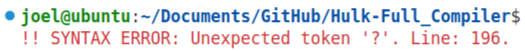
\includegraphics[width=0.7\textwidth]{images/parser_errors.png}
\caption{Error en parser}
\label{fig:errores_yacc}
\end{figure}

\subsection{Generador de lexer propio. NFA y DFA}

Como un \textit{lexer} clásico recibe una cadena de caracteres y genera una lista de tokens definidos
por las expresiones regulares que describen el lenguaje. El flujo general se basa en:

\begin{enumerate}
    \item Crear los autómatas finitos no deterministas (NFA) de cada expresión regular.
    \item Construir el autómata de la unión de todos los NFAs para definir el lenguaje que reconocerá el lexer.
    \item Convertir el NFA de la unión a un DFA (autómata finito determinista).
    \item Generar la secuencia de tokens a partir del DFA construido.
\end{enumerate}

\subsubsection{Intérprete de expresiones regulares} 

\

\

El objetivo de este intérprete es construir un NFA a partir de una expresión regular. Cuenta con un 
\textit{parser} específico que, a partir de los tokens resultantes de tokenizar la expresión regular,
construye un árbol de sintaxis abstracta (AST). Este AST es la entrada del método para generar el NFA
correspondiente. Reconoce la siguiente sintaxis de expresiones regulares:

\begin{itemize}
    \item \textbf{ $|$ }: Unión.
    \item \textbf{ * }: Clausura.
    \item \textbf{ + }: Clausura positiva.
    \item \textbf{[ ]}: Conjunto.
    \item \textbf{[ $^{\wedge}$ ]}: Conjunto negado.
    \item \textbf{[ - ]}: Conjunto expandido.
    \item \textbf{ . }: Cualquier caracter.
\end{itemize}

\subsubsection{Algoritmo para transformar un NFA a un DFA} 

\ 

\

El algoritmo utiliza un método auxiliar para computar la $\epsilon$-clausura (estados alcanzables por
$\epsilon$-transiciones) de un conjunto de estados del NFA. 
El DFA tendrá en cada estado, subconjuntos de los estados del NFA.

El algoritmo comienza calculando la $\epsilon$-clausura del estado inicial del NFA y esa será 
el estado inicial del DFA. Luego, por cada símbolo del alfabeto, por cada estado del NFA en el estado actual del DFA, se crea un conjunto de 
estados nuevo, que serán el resultado de aplicar la función de transición del NFA al estado y símbolo dados. Entonces el siguiente estado del DFA 
será la $\epsilon$-clausura de dicho conjunto recién construido, y sus estados finales serán los que contengan al menos
un estado que era final en el NFA.

\subsubsection{Generación de tokens} 

\ 

\

Los estados finales del DFA contienen los posibles tokens con que puede coincidir la cadena.
En el proceso de construcción de un token se transita por el DFA mientras sea posible y, si se llega a un estado final,
se guarda el lexema que se está construyendo y la lista de tokens correspondiente al estado en cuestión. La construcción de un 
token se puede detener por dos razones: no hay ninguna transición disponible en el autómata o se encuentra un espacio en blanco. En ambos casos, se guarda el (los) último (s) 
que coincidió (coincidieron) y se reinicia el recorrido por el DFA, comenzando por el caracter que detuvo la máquina. Finalmente, se retorna el token que más prioridad tenga (en caso de 
tener varios tokens, sino se retorna el único que se tiene). 


\vspace{10pt}
\section{Análisis semántico}

Como se ha mencionado anteriormente, la entrada del \textit{chequeo semántico} es el nodo raíz del AST, que es donde comienzan los chequeos, utilizando el
patrón Visitor. La implementación de este patrón (ver Figura~\ref{fig:visitor}) contiene: 
\begin{itemize}
    \item \textbf{Funciones de visita para cada tipo de nodo del AST}: Para cada nodo hay una función que sabe analizarlo y aplicar las reglas semánticas correspondientes.
    \item \textbf{Lista de errores semánticos encontrados}: Se mantiene una lista de errores semánticos encontrados durante el análisis, que se reportan al usuario al finalizar el chequeo.
    \item \textbf{Cantidad de errores semánticos encontrados}: Longitud de la lista de errores encontrados (recordar que en C no se puede obtener el tamaño de un array dinámico, por lo que se debe mantener un contador)
    \item \textbf{Recolector de contextos}: Se encarga de recolectar todas las declaraciones de funciones y tipos en el contexto actual, antes de analizarlas
    \item \textbf{Nombre de la función actual}: Se mantiene el nombre de la función que se está analizando actualmente, para evitar tener que subir de nuevo en el AST cuando se necesite, como por ejemplo al usar: \textit{base(...)}
    \item \textbf{Tipo actual}: Similar al caso anterior e igualmente necesario para el ejemplo brindado, pues en el caso del uso de \textit{base(...)} se debe saber el tipo de la clase actual para poder buscar el método en algún ancestro.
\end{itemize}

\begin{figure}[h]
\centering
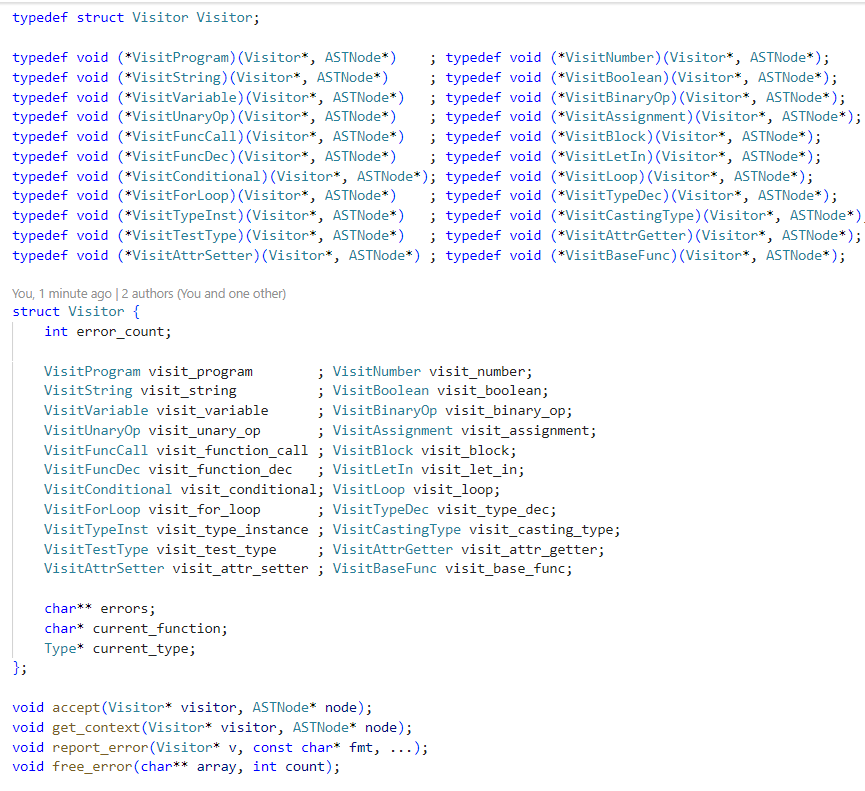
\includegraphics[width=1\textwidth]{images/visitor.png}
\caption{Implementación del patrón Visitor para el chequeo semántico}
\label{fig:visitor}
\end{figure}

El inicio del análisis se encuentra en el archivo \texttt{semantic.c}, donde primero se inicializa el visitor y luego se visita al nodo raíz del AST. La implementación de la función de
visita de ese nodo, primero realiza las declaraciones de tipos y funciones builtin del lenguaje, luego recoge el contexto del programa y finalmente visita cada uno de sus
descendientes. Al concluir el análisis, se imprimen en consola (con fuente en color Rojo) los errores reportados, y continúa el flujo del compilador. 
Para el chequeo semántico, cada nodo contará con un tipo de retorno, un ámbito (scope) y un contexto asociados (cada campo cumple una función específica y serán analizados posteriormente), y en caso de no
especificar lo contrario, se asumirá de aquí en adelante que en cada visita el ámbito y contexto padres son los del nodo padre (NULL en caso de la raíz).

Ahora se explicará detalladamente cada uno de 
los chequeos que se realizan a cada nodo.

\subsection{Análisis de expresiones básicas}

En la implementación, se consideran como expresiones básicas a los literales (números, cadenas, booleanos), operaciones unarias (!, -), 
operaciones binarias $(+, -, *, /, \%, ^, \&, |, ==, !=, <, >, <=, >=, @, @@)$, así como los bloques de expresiones.
\begin{enumerate}
    \item \textbf{Literales}: En el caso de los números y booleanos, las funciones de visita están vacías, pues no hay nada que chequear; sin embargo,
    en el caso de las cadenas, se verifica que los caracteres de escape utilizados (si los hay) sean correctos.
    \item \textbf{Operaciones unarias}: Primero se visita al nodo de la expresión hija y luego se chequea la compatibilidad del tipo de dicha expresión con
    la operación unaria dada. (La compatibilidad de tipos con operadores se explicará más adelante). Luego se actualiza el tipo de retorno del nodo según el operador.
    \item \textbf{Operaciones binarias}: Similiar a las operaciones unarias, se visitan primeros los nodos de las expresiones con las que se quiere operar y luego 
    se chequea la compatibilidad de ambos tipos con el operador binario dado (La compatibilidad de tipos con operadores se explicará más adelante). Luego se actualiza el tipo 
    de retorno del nodo según el operador.
    \item \textbf{Bloques de expresiones}: Similar al nodo raíz, el nodo bloque funciona como un mini programa, por lo cual se recolecta primero su contexto y luego se visita cada uno de sus 
    descendientes, manteniendo siempre el último visitado para poder al final actualizar el tipo de retorno del nodo bloque con el tipo de su último descendiente. Si el bloque esta vacío, automáticamente 
    se le otorga tipo de retorno \texttt{Void}.
\end{enumerate}

\textbf{Compatibilidad de tipos con operadores}: En el archivo \texttt{type.c} se definen todas las reglas de compatibilidad de tipos. En el arreglo \texttt{operator\_rules} (ver Figura~\ref{fig:operadores}) se almacenan las reglas para los 
operadores de la forma \{\texttt{tipo de la izquierda, tipo de la derecha, tipo de retorno, operador}\}. En caso que un operador pueda utilizarse con varios tipos, como es el caso del '==' por ejemplo, aparece una regla por cada
uso del operador. De esta forma, es más sencillo revisar la compatibilidad de tipos con operadores, pues solo se tienen que recorrer las reglas y comparar los tipos izquierdos y derechos (NULL para los unarios) según el operador.

\begin{figure}
\centering
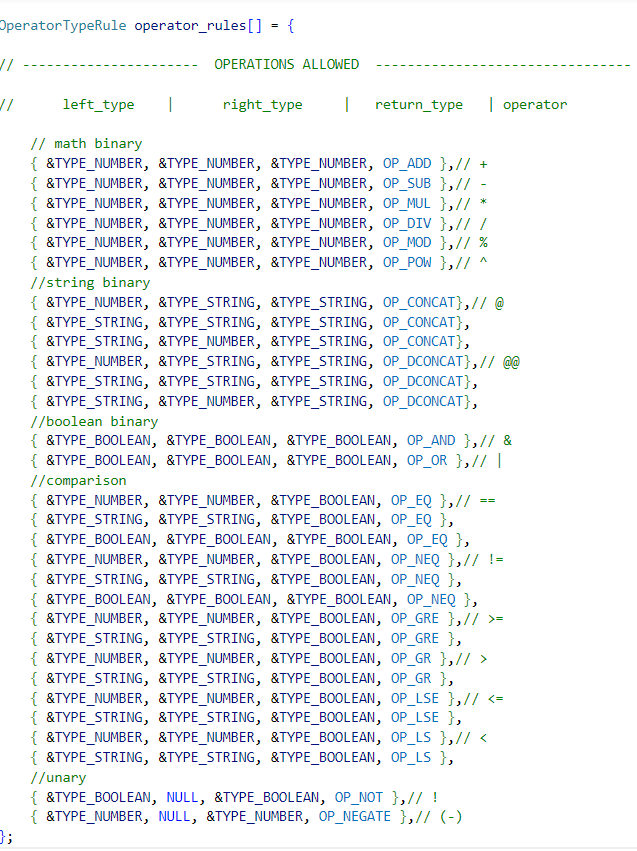
\includegraphics[width=1\textwidth]{images/op_rules.png}
\caption{Reglas para los operadores}
\label{fig:operadores}
\end{figure}

\textbf{Errores}: De manera general y como se expuso con anterioridad, en las expresiones básicas los errores más comunes son 
los respectivos a secuencias de escapes inválidas en cadenas e incompatibilidad con los operadores (ver ejemplo Figura~\ref{fig:errores_1}).
\begin{figure}[h]
\centering
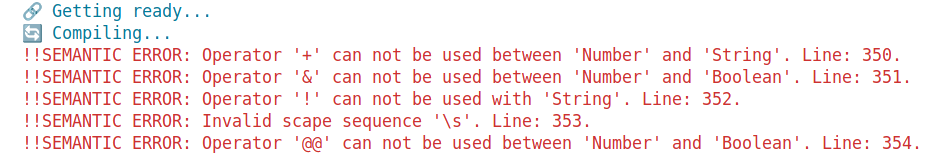
\includegraphics[width=1\textwidth]{images/basic_errors.png}
\caption{Errores comunes en expresiones básicas}
\label{fig:errores_1}
\end{figure}

\subsection{Análisis de variables y ámbitos (scopes)}

La revisión de variables, en general, contempla el chequeo de asignaciones, el uso de variables y
las expresiones \textit{let-in}. Para comprender mejor esta sección, se comenzará explicando la estructura 
de un \textit{scope} y las posibles acciones que se pueden realizar sobre él.

Un \textbf{scope}, en la implementación dada, es una estructura que contiene, a grandes rasgos, una tabla de
símbolos, una tabla de funciones y una tabla de tipos definidos, las cuales actúan como bases de datos para las
respectivas definciones en los distintos ámbitos del programa, además de una referencia al \textit{scope} padre.
Sobre los \textit{scopes} se pueden realizar diversas  acciones, iniciando claramente por su creación y
finalizando con su destrucción al concluir el chequeo semántico (en C la liberación de memoria es manual). Esas
acciones incluyen:
\begin{itemize}
    \item Guardar símbolos, funciones o tipos en las tablas.
    \item Buscar específicamente algún símbolo, función o tipo definidos.
    \item Inicializar tipos y funciones \textit{builtin}.
    \item Liberar memoria para cada tabla.
\end{itemize}

Luego de entender la estructura de los \textit{scopes}, se abordarán los distintos tipos de análisis realizados en el caso 
de las variables: 

\begin{enumerate}
    \item \textbf{Asignaciones}: La revisión comienza chequeando que el nombre dado a la variable no sea un \textit{keyword}, de lo contrario se reporta un error. También 
    con respecto a la variable, se verifica si fue tipada o no, y en caso que sí, se analiza que el tipo sea válido. Luego, se pasa al chequeo de la parte derecha de la asignación, 
    invocando su función de visita. Una vez termina de visitar la expresión de la derecha, se revisa la compatibilidad del tipo de dicha expresión con el tipo impuesto a la variable 
    (en caso de haber sido tipada, en otro caso no sucede nada) y se guarda en dependencia del operador de asignación. Si se utiliza \texttt{==} se crea un nuevo símbolo en el
    \textit{scope} padre, y en caso del operador destructivo \texttt{:=}, se busca el símbolo en la tabla de símbolos (de algún \textit{scope} ancestro) y se verifica que sean compatibles 
    los tipos de la inicialización y la reasignación. En caso que no, o que no se haya encontrado el símbolo se reportará error. En el caso del uso de asignación destructiva 
    el tipo de retorno del nodo es el mismo que el de la variable asignada (la cual toma el tipo de la expresión de la derecha si no fue tipada), y en caso contrario el retorno es \texttt{Void}.
    \item \textbf{Uso de variables}: Esta revisión es más sencilla, pues basta con buscar la variable en algún \textit{scope} ancestro y si no existe se reporta error.
    \item \textbf{Let-in}: Esta expresión esta compuesta por un conjunto de asignaciones y un cuerpo. Por tanto, la revisión consta de 
    visitar cada una de las asignaciones y luego visitar el cuerpo. El tipo de retorno es el mismo que el tipo de retorno del cuerpo.
\end{enumerate}

\textbf{Errores}: Como se expuso anteriormente, los errores detectados en estas revisiones son: tipo no definido al tipar una variable, 
incompatibilidad de tipos en asignaciones (en el caso de las que son tipadas), reasignar una variable que no ha sido inicializada antes, intentar reasignar una variable con un tipo incompatible 
con el tipo de su inicialización, variable indefinida, entre otros.  (ver ejemplo Figura~\ref{fig:errores_2}).
\begin{figure}[h]
\centering
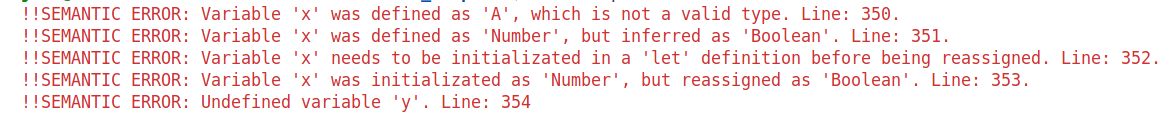
\includegraphics[width=1\textwidth]{images/var_errors.png}
\caption{Errores comunes en variables}
\label{fig:errores_2}
\end{figure}

\subsection{Análisis de funciones}

El análisis de funciones agrupa dos tipos de revisiones: chequeo de la declaración y chequeo del llamado. Como las funciones pueden declararse en cualquier sección del programa 
se necesita primero recoger el contexto de todas las declaraciones. Para eso se utiliza una estructura denominada \textit{context}.

El \textit{context}, al igual que el \textit{scope} sirve como una base de datos, pero dedicada a guardar los nodos de las declaraciones de funciones (o tipos, que se verán más adelante). 
Sobre un \textit{context} se puede: 
\begin{itemize}
    \item Guardar una declaración.
    \item Buscar una declaración.
\end{itemize}

Ahora se explicará cada una de las revisiones dichas anteriormente:
\begin{enumerate}
    \item \textbf{Llamado a funciones}: Lo primero que se se hace es visitar cada uno de los argumentos. Luego se busca la función en el \textit{context} y se revisa su declaración para que queden guardados sus 
    datos en el \textit{scope} (en caso de haber sido o estar en proceso de ser revisada, no sucede nada). Finalmente se chequea que la cantidad de argumentos y los tipos de los argumentos coincidan con la declaración 
    de dicha función y se actualiza el tipo de retorno del nodo del llamado con el guardado en el \textit{scope}.
    \item \textbf{Declaración de funciones}: Al igual que con la asignación de variables, se comienza revisando que el nombre de la función no sea una \textit{keyword}. Después se hace un pequeño chequeo para descartar que existan 
    nombres de parámetros repetidos. Luego se pasa a declarar en el \textit{scope} de la declaración cada uno de los parámetros para que sean accesibles en el cuerpo de la función, revisando primero que si son tipados, tengan un tipo válido. Al terminar 
    con los parámetros, se chequea el cuerpo, comenzando por ver si la función tiene un tipo de retorno definido, y en ese caso igualmente revisar que sea un tipo válido y más adelante que sea compatible con el tipo inferido del cuerpo; y luego se llama a su
    función de visita.
\end{enumerate}

\textbf{Errores}: Existen diversos tipos de errores que se detectan en estas revisiones: incompatibilidad de tipos en los parámetros, en el retorno, repetición de un 
mismo símbolo en los argumentos de una declaración, función no definida, cantidad de argumentos no compatible, entre otros (ver ejemplo Figura~\ref{fig:errores_3}).
\begin{figure}[h]
\centering
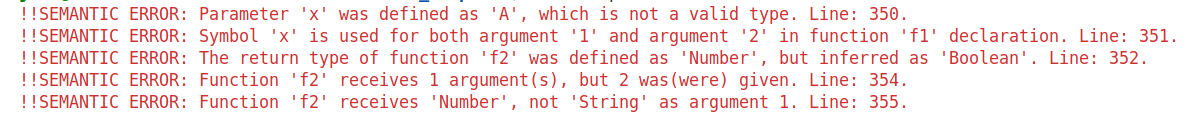
\includegraphics[width=1\textwidth]{images/func_errors.png}
\caption{Errores comunes en funciones}
\label{fig:errores_3}
\end{figure}

\subsection{Análisis de condicionales y ciclos}

La revisión de condicionales y ciclos se centra precisamente en revisar cada una de esas expresiones, además de un tipo 
especial de condicional: \textit{q-conditional}. A continuacón se explican cada una de ellas detalladamente: 
\begin{enumerate}
    \item \textbf{Condicionales}: Las condicionales tienen tres partes: condición, bloque para el \textit{if}, bloque para el \textit{else} 
    (el \textit{elif} es convertido automáticamente por el compilador a un \textit{else if}). La revisión ocurre secuencialmente por esas tres partes: 
    se visita el nodo de la condición y se verifica que su tipo de retorno sea booleano, sino se reporta error; luego se visita el bloque del \textit{if} 
    y más adelante el del \textit{else}. Entonces la expresión condicional toma como tipo de retorno el ancestro común más cercano entre los tipos de retorno 
    de ambos bloques. En caso de no tener bloque \textit{else}, se asume para ese caso un tipo por defecto para esta rama, que puede ser el mismo tipo que el del 
    primer bloque para los tipos \textit{builtin} (excepto \texttt{Object}) y \texttt{Null} para el resto. Este último genera que el valor de retorno de la condicional 
    sea el tipo del primer bloque pero \textit{nulleable}, por tanto, no se podrá utilizar luego en ningún caso donde se requiera ese tipo sin utilizar la sintaxis de \textit{q-conditional}, 
    que lo que hará será separar los casos en dos ramas: cuando el tipo sea \texttt{Null} y cuando sea exactamente el tipo deseado (se explicará luego).
    \item \textbf{Ciclos \textit{while}}: El ciclo \textit{while} es mucho más sencillo de verificar que las condicionales, pues solo admite un cuerpo. Por tanto, su chequeo se basa en 
    visitar la condición y reportar error si su tipo de retorno no es booleano, y más tarde visitar el cuerpo y actualizar el tipo de retorno del ciclo con el tipo de retorno del cuerpo.
    \item \textbf{Ciclos \textit{for}}: Este ciclo es más complejo que el anterior y comprende varias transformaciones importantes. Se chequea primero que los parámetros de la funcion \texttt{range} 
    cumplan los requisitos esperados (ser 1 o 2 parámetros numéricos). Luego el nodo \textit{for} se transforma en un \textit{let-in} para optimizar la generación de código y se revisa como tal: 
    \begin{lstlisting}[language=C]
    // ---> for original <---
    for (x in range(start, end)) {
        // cuerpo del for
    }

    // ---> Transformacion <---
    let _iter = start - 1 in 
    // _ al inicio evita que el usuario pueda usarla
        if (_iter += 1 < end) // por si no entra al while
            while (_iter += 1 < end)
                let x = _iter in {
                    // cuerpo del for
                }
    // Esta transformacion simula un iterable
    \end{lstlisting}
    \item \textbf{Condicionales \textit{q-conditional}}: Este tipo de condicional es una extensión al lenguaje que permite separar los casos de un tipo nulleable en dos ramas: una para el caso donde el es \texttt{Null} y otra donde es el tipo original no \textit{nulleable}. Posee 
    la siguiente sintaxis: 
    \begin{lstlisting}[language=C]
    if?(<expression>) // variable
        <expression> // asumiendo Null
    else 
        <expression> // asumiendo tipo original
    \end{lstlisting}
    Por detalles de tiempo, esta nueva sintaxis se mantiene en una versión inicial donde solo es capaz de recibir como argumento una variable. No obstante, como en una variable se puede guardar cualquier expresión, pues es completamente funcional. Al igual que las condicionales, su tipo de 
    retorno es el ancestro común más cercano entre ambos bloques (son obligatorios ambos bloques). Fuera de la expresión \textit{q-conditional} la variable mantiene su estado original, así que si se desea que se comporte como el tipo no \textit{nulleable} debe usarse dentro del bloque \textit{q-conditional} 
    necesariamente.
\end{enumerate}

\textbf{Errores}: Los errores en estas revisiones son pocos, principalmente cuando las condiciones no son booleanas y cuando hay incompatibilidad con los parámetros de la función range. (ver ejemplo Figura~\ref{fig:errores_4}).
\begin{figure}[h]
\centering
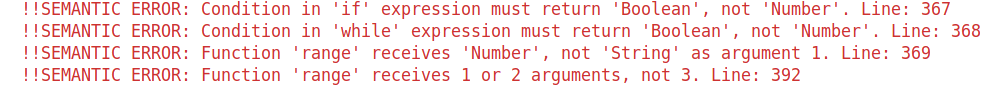
\includegraphics[width=1\textwidth]{images/cond-loop_errors.png}
\caption{Errores comunes en condicionales y ciclos}
\label{fig:errores_4}
\end{figure}

\subsection{Análisis de Tipos}

El análisis de tipos es el chequeo más abarcador de esta sección. Comprende la declaración de tipos, instancias de tipos, obtención y modificación de atributos, operaciones de chequeo y conversión de tipos, y el caso especial de la función \textit{base}.

Para comprender mejor estos análisis, es necesario explicar la estructura \texttt{Type} en el programa. Esta estructura es la que maneja, en todo momento del chequeo semántico, los tipos de retorno de las expresiones. Posee, de manera general, 
un nombre, un padre, los tipos de los parámetros que recibe su constructor, así como la cantidad, y además tiene un campo para acceder a su declaración y poder tener referencia a sus atributos y métodos. Sobre un \texttt{Type} se pueden hacer distintas 
operaciones: 
\begin{itemize}
    \item Crear un nuevo tipo
    \item Saber si el tipo es \textit{builtin}
    \item Saber si dos tipos son iguales
    \item Saber si un tipo es ancestro de otro
    \item Saber el ancestro común más cercano entre dos tipos 
    \item Saber si dos tipos están en la misma rama de la jerarquía de tipos 
    \item Obtener el tipo \textit{nulleable} asociado
\end{itemize}

Una vez comprendido el funcionamiento de un \texttt{Type} se explicará cada uno de los chequeos que se pueden realizar:
\begin{enumerate}
    \item \textbf{Chequeo de tipos}: Este chequeo se puede realizar mediante el operador \textit{is}. Primero se visita al nodo de la expresión que se quiere chequear y luego se revisa que el tipo por el que se pregunta exista en el \textit{scope}, o en última 
    instancia en el \textit{context}. De no ser así, se reportará error.
    \item \textbf{Conversión de tipos}: Al igual que el chequeo de tipos, se visita la expresión y se revisa que el tipo a convertir exista o bien en el \textit{scope} o en el \textit{context}. Además, hay una verificación extra que detecta si el tipo de 
    la expresión y al que se quiere convertir estén en la misma rama de la jerarquía de tipos, de lo contrario se reporta también error.
    \item \textbf{Instancia de tipos}: Las instancias de tipos, de cierta manera, son similares a los llamados de funciones, por lo tanto su chequeo es igual, solo que en vez de buscar funciones definidas se busca tipos. Incluso los errores reportados son 
    los mismos (solo cambia \textit{function} por \textit{type} en la mayoría de los mensajes).
    \item \textbf{Declaración de tipos}: La declaración de tipos tiene un chequeo robusto, pues puede dar lugar a decenas de errores distintos. Se comienza revisando que no exista herencia circular, para lo cual se mantiene una lista estática a la que se tiene acceso y 
    que almacena nombres de tipos. Se chequea que el nombre del padre no esté en esa lista (en caso que sí se reporta la circularidad), y luego se añade. Esa lista se vacía nuevamente cuando se inicie el chequeo del cuerpo de la declaración del tipo. Sobre los parámetros del 
    constructor se realizan las mismas verificaciones que en la declaración de una función. Con respecto a la herencia, se verifica, en caso de tener padre, que dicho tipo sea válido, sino se reporta error, y además, se revisa la compatibilidad de los parámetros, que incluye 
    añadir a la declaración del tipo los parámetros que recibe el constructor del padre en caso de no especificar los suyos propios, o verificar que se haya dado una inicialización correcta al padre a partir de los parámetros que reciba el tipo en cuestión. Con eso se da por concluida 
    la revisión de la cabecera del tipo y se comienza la revisión del cuerpo. Lo primero es recoger un contexto interno, que incluye inicializaciones de campos y métodos. Luego se visita primero cada una de las inicializaciones y luego los métodos (antes de visitarlos se declara en el
    \textit{scope} interno del tipo la variable especial \textit{self} del mismo tipo que el declarado). Para estos últimos, cabe resaltar que además de los chequeos habituales de las declaraciones de funciones, también se verifica que cumpla con la signatura de la declaración previa en
    un ancestro (de haberla). Finalmente se crea el tipo y se le asocia dicho nodo de la declaración para poder acceder luego a sus miembros.
    \item \textbf{Obtención de atributos}: Para obtener atributos o métodos de un tipo específico, se emplea la notación punto: \texttt{instance.member}. Por tal motivo, primero se visita el nodo que representa la instancia del tipo. Una vez que se tiene la instancia, se verifica que el miembro 
    solicitado esté definido en el tipo de la instancia, en caso contrario se reporta error. Finalmente, si existe el miembro, se visita su nodo y se actualiza el tipo de retorno del nodo principal, con el tipo de retorno del miembro asociado.
    \item \textbf{Modificación de atributos}: Para modificar atributos se usa la misma sintaxis de notación punto: \texttt{instance.member := value}. Igualmente se visita el nodo de la instancia y se verifica que contenga el atributo a modificar, de lo contrario se reporta error. Luego 
    se visita el nodo de la expresión que constituye la modificación que se quiere realizar. Luego se revisa que el tipo de dicha expresión sea descendiente del tipo con que fue inicializado el atributo, y si no, también se detecta error.
    \item \textbf{Función \textit{base}}: Es una función especial, que necesita conocer el método y el tipo actuales, ambos datos guardados en el \textit{visitor}. El chequeo comienza tomando esos datos y buscando el tipo más próximo que posee una declaración para dicha función. En caso de 
    no existir, se reporta error. Luego, como es, en esencia, un llamado a función, debe chequearse como tal. Esto se logra creando un nodo auxiliar de tipo \texttt{NODE\_FUNC\_CALL} con el nombre de la función que se encontró y los argumentos que recibía \textit{base}. Luego se visita ese nodo y cualquier 
    error que pueda existir quedará registrado. Finalmente, el tipo de retorno de \textit{base} es el tipo de retorno de la función que invoca.
\end{enumerate}

\textbf{Errores}: Los errores en el manejo de tipos son muy diversos. Existen errores en las declaraciones que son similares a los de las declaraciones de funciones, así como en las instancias que son parecidos a los llamados. Además, tiene errores propios, referentes a la herencia y referencias circulares, 
heredar de tipos \textit{builtin}, redefinición de atributos y métodos, acceder a los atributos desde fuera de la instancia (son privados), atributo o método inexistente en un tipo específico, conversión de tipos inválida, intentar modificar un atributo asignando un valor de tipo distinto al de su inicialización, 
entre otros (ver ejemplo Figura~\ref{fig:errores_5}).
\begin{figure}[h]
\centering
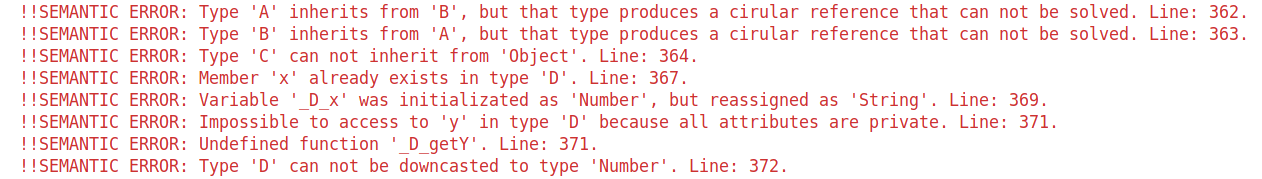
\includegraphics[width=1\textwidth]{images/type_errors.png}
\caption{Errores comunes en el manejo de tipos}
\label{fig:errores_5}
\end{figure}

\subsection{Inferencia de tipos. Unificación}

La implementación propuesta del compilador de HULK, posee una inferencia de tipos fuerte, es decir, el tipado explícito solo es necesario cuando el programa detecte que es incapaz de inferir el tipo. Existe una primera inferencia simple y sencilla, basada en un conjunto de reglas básicas: 
\begin{itemize}
    \item Los literales son los más fáciles de inferir, ya que su tipo proviene directamente del analizador. Las expresiones aritméticas también son fáciles, ya que su tipo siempre es \texttt{Number}. Asimismo, los operadores de cadena y booleanos son sencillos.
    \item El tipo de expresiones complejas que tienen un cuerpo de expresión se determina por el tipo de dicho cuerpo. Este es el caso de \textit{let-in}, \textit{while} y \textit{for}.
    \item El tipo de un bloque de expresión es el tipo de la última expresión del bloque.
    \item El tipo de una invocación de función o método es el tipo de su cuerpo.
    \item El tipo de expresiones que tienen más de una rama (\textit{if}) es el ancestro común más cercano de los tipos de cada rama, o, en última instancia, \texttt{Object}.
\end{itemize}

Más allá de esa inferencia simple, también existe una mucho más compleja, referente a los parámetros de funciones y tipos. Esos parámetros no tienen asociado una expresión en las declaraciones, por tanto, si no están tipados, es imposible inferir su tipo basado solo en las reglas anteriores. Hay que deducirlo entonces 
a partir de su uso. Para eso, se ha diseñado una especie de motor de unificación, el cual intenta asignar un tipo específico a un parámetro. 

Para su correcto funcionamiento, cada nodo del AST tiene un campo \textit{derivations}, que puede ser visto como una lista de nodos. Cada nodo en esa lista repesenta una expresión de la cual el nodo principal podría haber obtenido un tipo \texttt{Any}, que es el que se le asigna inicialmente a los parámetros no tipados. 

Dado que el programa solo asigna directamente \texttt{Any} a los parámetros y al retorno de las funciones que aún se están chequeando, cualquier expresión cuyo tipo de retorno sea \texttt{Any} necesariamente depende de un parámetro o un llamado a una de esas funciones. Dicho esto, el unificador se encargará de buscar la raíz del tipado \texttt{Any}, es decir, la función o el parámetro específico que derivó en la expresión más grande.
Para hacerlo, simplemente toma un nodo y, o bien es un parámetro o una función, o es una expresión que contiene alguno. Si se cumple lo primero, directamente se actualiza su tipo con el que se quiere unificar, y en otro caso se intenta unificar cada una de sus \textit{derivations}. Luego de unificar 
un nodo, debe visitarse nuevamente para expandir los cambios producidos.

Todo este procedimiento de unificación necesita claramente un tipo con el cual unificar. Hay distintas maneras de obtener dicho tipo, en dependencia del nodo actual. Algunos pueden pedir unificación con un tipo directamente, como es el caso de las condicionales, que intentan unificar la expresión de la condición con el tipo \texttt{Boolean}. 
Sin embargo en otros casos, se necesita un proceso para obtener el tipo, antes de intentar unificarlo. Ese es el caso de las expresiones aritméticas, o los llamados a funciones e instancias de tipos. Otro de los más destacados, es el uso de parámetros en notación punto, donde la inferencia debe buscar entre todos los tipos cuál es 
el que tiene el miembro requerido e intentar unificar con ese (siempre se queda con el ancestro común más cercano que implemente el método entre todos los que implementan el método, o reportará error).

\  

\textbf{Errores}: Los errores de inferencia se resumen en dos tipos: se infirieron dos tipos de ramas distintas de la jerarquía de tipos, o simplemente no se pudo inferir un tipo (ver ejemplo Figura~\ref{fig:errores_6}).
\begin{figure}[h]
\centering
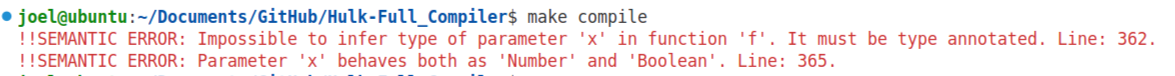
\includegraphics[width=1\textwidth]{images/inference_errors.png}
\caption{Errores comunes en la inferencia de tipos}
\label{fig:errores_6}
\end{figure}

\vspace{10pt}
\section{Generación de Código}

La fase final del compilador es la generación de código intermedio (LLVM). En este fase, se utilizó el framework de C para LLVM, a través del cual se genera el archivo \texttt{output.ll}. En esta sección no se abordará específicamente la sintaxis de ese lenguaje, sino que se explicarán las ideas y abstracciones principales que permitieron llevar 
un lenguaje de alto nivel como HULK a un lenguaje intermedio. 
\vspace{10pt}
\begin{thebibliography}{9}
\bibitem{aho06}
Aho, A.V., Lam, M.S., Sethi, R., Ullman, J.D.: 
Compilers: Principles, Techniques, and Tools (2nd Edition). 
Addison-Wesley (2006)

\bibitem{appel98}
Appel, A.W.: Modern Compiler Implementation in C. 
Cambridge University Press (1998)

\bibitem{llvm}
Lattner, C., Adve, V.: 
LLVM: A Compilation Framework for Lifelong Program Analysis \& Transformation. 
CGO 2004, LNCS 3161, Springer (2004)
\end{thebibliography}
\end{document}